\section{Riemannian Laplace Approximation}
In comes the Riemanninan Laplace approximation. The idea here is to use samples from the laplace approximation, but take into account the curvature of the loss landscape, such that parameters which are far away from our MAP solution in terms of the the curvature of the loss landscape get penalized.

For this purpose it is beneficial to define the loss manifold as $\mathcal M = g(\theta) = [\theta, \mathcal L(\theta)]$. Let us then consider a curve $c:[0,1] \mapsto \Theta$ on the parameter space parameterized by $t\in [0,1]$ \footnote{In the literature the curve is on the manifold. The function $g(\theta)$ gives a one-to-one correspondence between $\Theta$ and $\mathcal M$, so we can think of any operation taking place on either of the two, as we like.}. Then if $\dot c(t)$ is the time derivative of the curve, and $\bm J_{c(t)} = \left. \frac{\partial g}{\partial \theta} \right \vert_{\theta = c(t)}$ is the Jacobian of $g$ taken in the point $\theta=c(t)$, following \cite{Hauberg2025} we can write out the length of the curve as 
\begin{align*}
    \text{Length}_\mathcal M (c) 
    &= \int_0^1 \left\Vert \frac{d}{dt} g(c(t)) \right\Vert dt\\
    &= \int_0^1 \left\Vert \bm J_{c(t)} \dot c(t) \right\Vert dt\\
    &= \int_0^1 \sqrt{\dot c(t)^\top  \bm J_{c(t)}^\top \bm J_{c(t)} \dot c(t)} dt.
\end{align*}
Here we can use that $\bm J_{c(t)} = [\mathbb I_d, \nabla_\theta \mathcal L(\theta)]$ to define the \emph{Riemannian matric} on $\mathcal M$ as 
\begin{equation}
M(\theta) = \bm J_{c(t)}^\top \bm J_{c(t)} = \mathbb I_d + \nabla_\theta \mathcal L(\theta) \nabla_\theta \mathcal L(\theta)^\top    \label{eq:riemann_metric}
\end{equation}
This notion of distance induces two defintions. 

First the geodesic, which is the which is a shortest curve between two points $(\theta_0, \theta_1)$ on the manifold: 
\begin{align}
    c^\ast=& \,\, \underset{c}{\text{argmin}} \, \text{Length}_\mathcal M (c) \\
    & \,\,\text{subject to } c(0) = \theta_0 \text{ and } c(1) = \theta_1 \label{eq:geodesic}
\end{align}
Finding the geodesic between two points corresponds to solving a boundary value problem for a differential equation and is generally computationally expensive. 
The directional vector at time 0, given by $\dot{c}^\ast_0$ uniquely determines the curve (as we shall shortly see), and this motivates the definition of the Log-map, which takes two points $(\theta_0, \theta_1)$ in parameters space as input and returns a vector in parameter space\footnote{Corresponding to the previous note: the literature defines log Log-map on the manifold and returns a directional vector in $\Theta \times \mathbb R$}:
\begin{equation*}
    \text{Log}_{\theta_0}(\theta_1) \coloneqq \dot{c}^\ast(0)
\end{equation*}
The Log-map is thus the initial velocity of the geodesic that starts from $\theta_0$ and reaches $\theta_1$ in one time unit \cite{fröhlich2021bayesianquadratureriemanniandata}.
The "inverse" of this mapping is the Exp-map, which given a starting point $\theta^\ast$ and a directional vector $v$ returns the point that is reached by moving in direction $v$ from $\theta^\ast$ on the loss manifold for one time unit. That is, if 
$\text{Exp}_{\theta_0}(v) = c(1)$ then $v = \text{Log}_{\theta_0}(c(1))$.
The Exp-map corresponds to solving the initial value problem for the differential equation \cite{bergamin2023riemannian}:
\begin{equation}
    \ddot{c}(t)=-\nabla_{\theta}\mathcal{L}(c(t))\left(1+\nabla_{\theta}\mathcal{L}(c(t))^{-1}\nabla_{\theta}\mathcal{L}(c(t))\right)^{-1}\langle\dot{c}(t),\mathbf{H}_{\theta}[\mathcal{L}](c(t))\dot{c}(t)\rangle.
\end{equation}
It then holds that $\text{Exp}_{\theta_0}(\text{Log}_{\theta_0}(v)) = v.$
Note however that the Log-map is not uniquely defined, so the reverse does not necessarily hold. Furthermore, it holds that if $c^\ast$ is the geodesic between $\theta_0$ and $\theta_1$, and $v=\text{Log}_{\theta_0}(\theta_1)$, then for any $t \in [0,1]$ it also holds that $c^\ast(t\cdot v) = \text{Exp}_{\theta_0}(t\cdot v)$.
In this paper, all IVP's are solved numerically using the \verb|emukit| package \cite{emukit2023}.

\begin{figure}[ht]
    \centering
    \subfloat[Laplace approximation to the banana distribution]{
        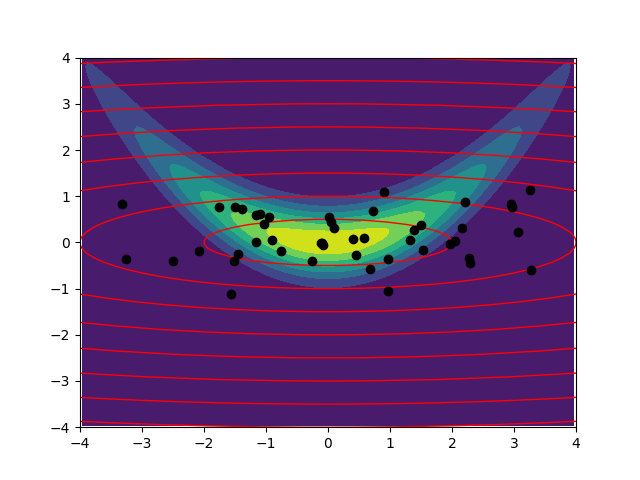
\includegraphics[width=.31\linewidth]{report/figures/banana_distr_contour_laplace.png}
        \label{fig:banana_distr_contour_laplace}
    }
    \hfill
    \subfloat[Riemannian Laplace samples from banana distribution]{
        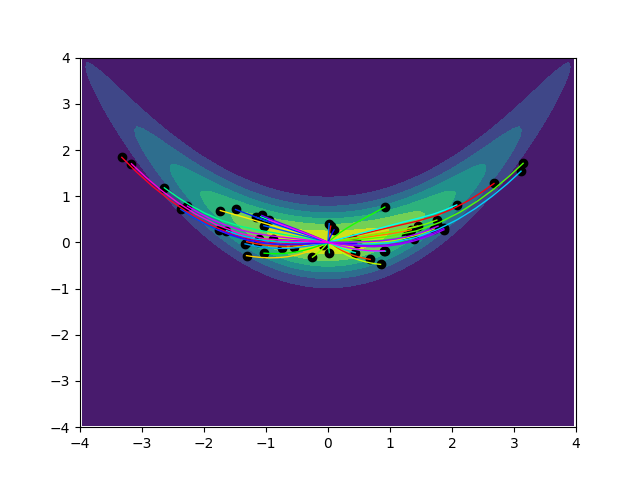
\includegraphics[width=.31\linewidth]{report/figures/banana_distr_contour_riemannshots.png}
        \label{fig:banana_distr_contour_riemannshots}
    }
    \hfill
    \subfloat[Riemannian Laplace approximation for UFA]{
        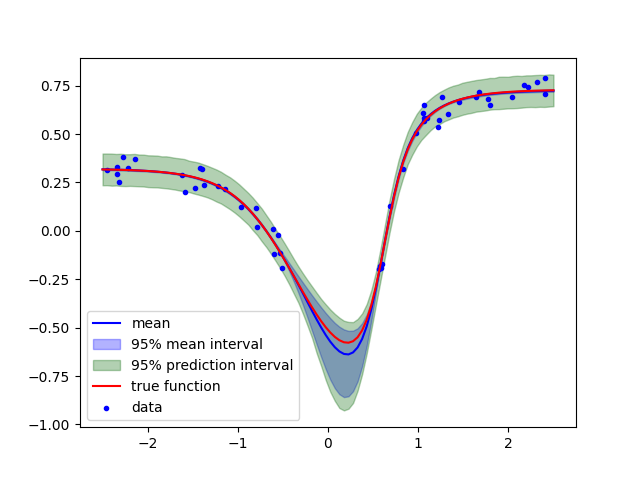
\includegraphics[width=.31\linewidth]{report/figures/UFA_riemannian_subspace_rank2.png}
        \label{fig:UFA_riemannian_subspace_rank1}
    }
    \caption{Riemannian Laplace approximations}
    \label{fig:riemannian_laplaceapprox}
\end{figure}

In figure \ref{fig:banana_distr_contour_laplace}, 50 samples from the Laplace approximation together with corresponding red isocurves for the Laplace density are overlayed the Banana distribution. The Exp-map of the same samples are seen in figure \ref{fig:banana_distr_contour_riemannshots} together with their corresponding geodesics. In figure \ref{fig:UFA_riemannian_subspace_rank1}, we see the resulting UFA with prediction bands, as given by 10 samples along the first eigendirection of the Riemmanian Laplace approximation.

